\documentclass{beamer}
 
\usepackage[utf8]{inputenc}
\usepackage{multicol}

\usetheme{Szeged}
\usecolortheme{beaver} 
 

\title{Lerntraining Software}
\subtitle{Python}
\author{Sophie Aerdker}
\institute{Ruhr-Universit\"at Bochum}
\date{Mai 2018}
 
 
 
\begin{document}
 
\frame{\titlepage}
\begin{frame}
\frametitle{Table of Contents}
	\begin{multicols}{3}
 		 \tableofcontents
	\end{multicols}
\end{frame}

\section{Overview}

\begin{frame}
\frametitle{Overview}
	Python is ...\\
	\begin{itemize}
		\item interpreted
		\item interactive 
		\item object-oriented 
		\item a beginners language!
	\end{itemize}
	
	This tutorial is mostly inspired by \url{https://www.tutorialspoint.com/python/index.htm}. \\ Much of what you learn here you will find there!
\end{frame}

\begin{frame}
\frametitle{This tutorial}
	\begin{itemize}
		\item Introduction to basic programming techniques in \texttt{python} as well as an outlook to advanced methods
		\item There are exercises between some sections, where you can try out what you have learned bevor
		\item The slices are english, as most of the documentation so that you become familiar with the technical terms
		\item It will be a tight program, so don't worry if you don't understand everything directly! If you are intersted in programming, you can read a lot more in detail. I will present some literature and helpful websites later. 
		\item I will present python2 - what is not the latest standard, but for this tutorial the differences are not relevant.
	\end{itemize}
\end{frame}



\subsection{Setup}

\begin{frame}
\frametitle{For you at home, here \texttt{python} is already installed!}
	\begin{itemize}
		\item Check if \texttt{Python} is already installed: open a terminal and type "python", if not:
		\item Linux: type \texttt{sudo apt-get install python} or \texttt{sudo apt-get install python3} for python3
		\item Windows: \url{https://www.python.org/downloads/windows/}
	\end{itemize}
	Using \textit{Anaconda} distribution, which makes it easy to install packages:
	\begin{itemize}
		\item \url{https://www.anaconda.com/download/}
	\end{itemize}
	Or use an IDE like \textit{eclipse} or \textit{Visual Studio}
\end{frame}

\section{First Steps}
\subsection{Hello World!}

\begin{frame}
\frametitle{ Hello World!}
	\begin{columns}[T]
		\begin{column}[T]{7cm}
			\begin{itemize}
				\item open an editor 
				\item type: \texttt{print "Hello World!"}
				\item save it as "HelloWorld.py" under ...
				\item open a terminal and go to your directory with cd ...
				\item type: \texttt{python HelloWorld.py}
			\end{itemize}
		\end{column}
		\begin{column}[T]{5cm}
			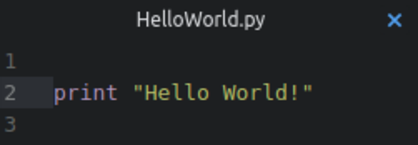
\includegraphics[width = 1\textwidth]{HelloWorld.pdf}
		\end{column}
	\end{columns}
\end{frame}


\begin{frame}
\frametitle{Simple Calculations}
	\begin{columns}[T]
		\begin{column}[T]{7cm}
			\begin{itemize}
				\item now type e.g. \texttt{x = 5} and \texttt{y = 10} under your print statement
				\item type \texttt{print} and a calculation using +,-,*,/
				\item save the file, go to your terminal and type \texttt{python HelloWorld.py} or press $\uparrow$
				\item What is the result of \texttt{x/y}?
				\item Instead you can try the interactive mode: Open a terminal and type \texttt{python}. Now you can type the mathematical expressions directly into the terminal and use it as an calculator.
			\end{itemize}
		\end{column}
		\begin{column}[T]{3cm}
			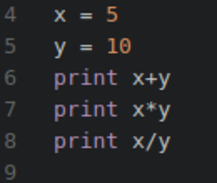
\includegraphics[width = 1\textwidth]{SimpleCalculations.pdf}
		\end{column}
	\end{columns}
\end{frame}

\section{Variable Types}

\begin{frame}
\frametitle{Variable Types}
	Python has five basic data types:
	\begin{itemize}
		\item Numbers, like 5 and 10
		\item Strings, like "Hello World!"
		\item Lists, 
		\item Dictionary, sometimes very useful but is not presented here
		\item Tuple
	\end{itemize}
	Data types can be stored in variables:
	\begin{itemize}
		\item  \texttt{x = 10}
		\item  \texttt{gravConstant = 9.81}
		\item  \texttt{s = "Hello World!"}
		\item  \texttt{name = "Sophie"}
	\end{itemize}
\end{frame}

\subsection{Numbers}

\begin{frame}
\frametitle{Basic numerical types with some examples}
	\begin{tabular}{c|c|c}
		Type & Examples & Comment \\ \hline
		int  & 3, -42 &  signed integer $ \leq 2,147,483,647$\\
		long & 51924361L & signed integer $>2,147,483,647$ \\
		float & 3.14, 3.0+e10, 0. & floating point real values \\
		complex & 42.0j, 2.+0.3j & complex numbers, imaginary unit j
 	\end{tabular}
 	
 	\begin{alertblock}{Integer Division}
 		The statement \texttt{5/10} is interpreted as an integer! Thus, its integer division is 0. Instead type 			\texttt{5./10.} to obtain a float-type value.
 	\end{alertblock}
 	\begin{block}{Boolean}
 		The result of a comparison which is \texttt{True} or \texttt{False} is called Boolean. \texttt{True} and 			\texttt{False} are special versions of 1 (or any non-zero/null value) and 0, respectively. You can use them in arithmetic contexts.
 	\end{block}	
\end{frame}

\subsection{Operators}

\begin{frame}
\frametitle{Arithmetic and Comparison Operators}
	\begin{tabular}{cc|c}
		\multicolumn{2}{c|}{Operator} & Examples  \\ \hline
		+ & Addition & 5+10 = 15  \\
		- & Subtraction & 10-5 = 5  \\
		* & Multiplication & 10*5 = 50   \\
		/ & Division & 10/5 = 2, 5/10 = 0, 5./10. = 0.5 \\
		** & Power & 10**5 = 10,000 \\
		\% & Modulus & 10\%5 = 0, 5\%10 = 5 \\
		// & Floor Division & 9.//2. = 4.0 \\ \hline
		== & equal & 5==10 is False, 5==5 is True  \\
		!= & not equal & 5!=10 is True, 5!=5 is False  \\
		$>$ & greater than & 10 $>$ 5 is True  \\
		$<$ & less than & 10 $<$ 5 is False \\
		\multicolumn{2}{l|}{$<=$ or $>=$} & 10 $>=$ 5 is True, 5 $<=$ 5 is True \\
 	\end{tabular}	
\end{frame}

\begin{frame}
\frametitle{Asignment Operators}
	\begin{tabular}{c|p{5cm}|p{3cm}}
		Operator & Description & Example  \\ \hline
		= & Assigns values from the right side to the left side & x = 5+10 \\
		+= & Adds right operand to the left one AND assigns the result to the left operand & x += 1 is equivalent to x = x + 1 \\ \hline	
		-= &  \multicolumn{2}{c}{x -= 1  is equivalent to x = x-1} \\
		*= &  \multicolumn{2}{c}{x *= 2 is equivalent to x = x*2} \\
		/= &  \multicolumn{2}{c}{x /= 2 is equivalent to x = x/2 }\\
		**= & \multicolumn{2}{c}{x **= 2 is equivalent to x = x**2} \\
		\%= &  \multicolumn{2}{c}{x \%= 2 is equivalent to x = x\%2 }\\
		//= &  \multicolumn{2}{c}{x //= 2 is equivalent to x = x//2 }\\ 	
 	\end{tabular}	
\end{frame}

\begin{frame}
\frametitle{Other Operators}
	\begin{alertblock}{Bitwise operators} 
		which perform bit by bit operations like: binary AND, OR, shifting
	\end{alertblock}
	\begin{alertblock}{Logical operators} 
		\texttt{not} , \texttt{or} , \texttt{and} \\
	\end{alertblock}
	\begin{alertblock} {Membership operators} 
		\texttt{in} and \texttt{not in} \\test the membership in a \textit{sequence} such as lists or strings
	\end{alertblock}
	\begin{alertblock}{Identity operators} 
		\texttt{is} and \texttt{is not} \\compare the memory locations of two objects, you can often use them like \texttt{==} and \texttt{!=}	for example in \textit{if-statements}
	\end{alertblock}
\end{frame}

\subsection{Strings}

\begin{frame}
\frametitle{Strings and string formatting}
	\begin{itemize}
		\item In Python there is no difference between 'chars' and "strings", single and double quotes are treated the same.
		\item You can create strings simply by putting characters in quotes: str = \texttt{"Hello World!"}
	\end{itemize}
	You can format strings using the string formatting operator '\%': \\
	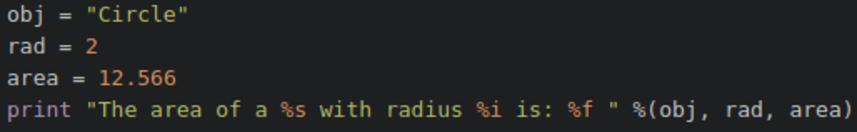
\includegraphics[width = 0.9\textwidth]{StringFormat.pdf} \\
	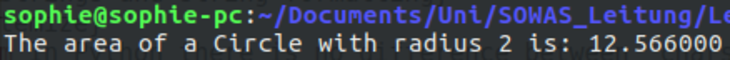
\includegraphics[width = 0.8\textwidth]{StringFormatOutput.pdf}
	
	You can find a table with format symbols here: \url{https://www.tutorialspoint.com/python/python_strings.htm}
\end{frame}


\section{Decision Making}

\begin{frame}
\frametitle{If-statements}
	\begin{columns}[T]
	\begin{column}[T]{5cm}
			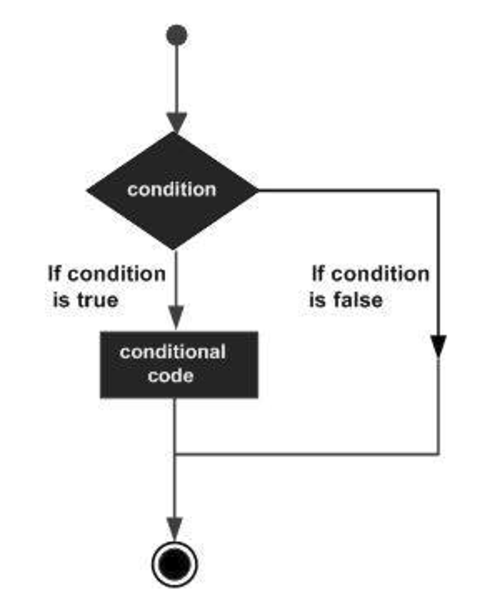
\includegraphics[width = 1\textwidth]{DecisionMaking.pdf}
		\end{column}
		\begin{column}[T]{3cm}
			use \texttt{if} and \texttt{else} conditions to execute a specific code if a condition is TRUE or to jump to the next (or another conditional) code otherwise	
		\end{column}	
	\end{columns}
\end{frame}

\begin{frame}
\frametitle{Example}
	\begin{columns}[T]
		\begin{column}[T]{0.6\textwidth}
			Some \texttt{if}, \texttt{elif}, \texttt{else} statements to compare the values x and y:\\
			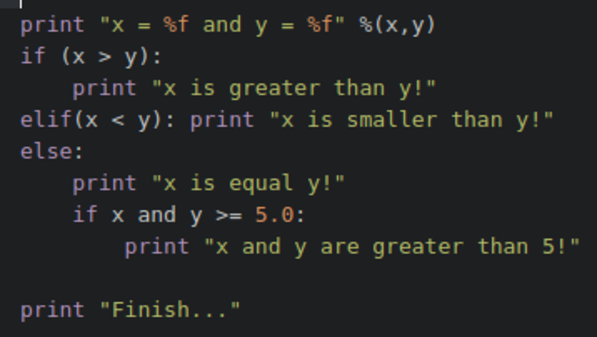
\includegraphics[width = 1\textwidth]{Comparison.pdf}
		\end{column}
		\begin{column}[T]{0.4\textwidth}
			Output for different values of x and y:\\
			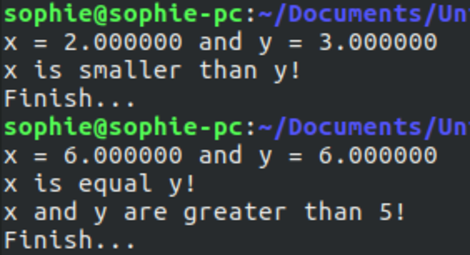
\includegraphics[width = 1\textwidth]{OutputComparison.pdf}	
		\end{column}	
	\end{columns}
	\begin{alertblock} {Syntax} 
		The conditional code has to be intended or stands in a line (only possible for one statement) with the condition. IDEs and many editors do this automatically.
	\end{alertblock}
\end{frame}


\begin{frame}
\frametitle{Exercises}
	\begin{itemize}
		\item Write the program \texttt{EvenOdd.py} which returns wether a variable is even or odd! \\ Use operators and condition statements and print the value as well as the result!
		\item Write the program \texttt{CharInString.py} which returns wether the string \texttt{"Hello World!"} contains a specific letter (a so called char)! \\ Use membership operators and the program should be case sensitive to keep it simple.
		\item Bonus: Use a string method (\url{https://www.tutorialspoint.com/python/python_strings.htm}) to make \texttt{CharInString.py} case insensitive
	\end{itemize}
\end{frame}


\section{Lists}

\begin{frame}
\frametitle{Lists}
	A list contains several items like strings or numbers, you can easily create a list with [] and ,-separated items: 
	\begin{itemize}
	\item \texttt{fruits = ["apple", "banana", "strawberry"]}
	\item \texttt{numbers = [1,1,2,3,5,8]}
	\end{itemize}
	The items in a list can be of different types:
	\begin{itemize}
	\item \texttt{book = ["title", "physics", 1997]} 
	\end{itemize}
	You can access an item in a list by its index:
	\begin{columns}[T]
	\begin{column}[T]{5cm}
		\begin{itemize}
			\item \texttt{fruits[1]} is \texttt{"banana"} 
			\item \texttt{numbers[3]} is \texttt{3}
		\end{itemize}
	\end{column}
	\begin{column}[T]{5cm}
		\begin{itemize}
			\item \texttt{fruits[0]} is \texttt{"apple"} 
			\item \texttt{numbers[-1]} is \texttt{8}
		\end{itemize}
	\end{column}
	\end{columns}
	\begin{alertblock}{Index}
	The index of a list starts with 0! You can use negative indices, too!
	\end{alertblock}
\end{frame}

\begin{frame}
\frametitle{Manipulating Lists}
	You can use the index to change an item at the index position:
	\begin{itemize}
	\item \texttt{fruits[0] = "mango"} results in \texttt{["mango", "banana", "strawberry"]}
	\end{itemize}
	You can delete an item at a specific position:
	\begin{itemize}
	\item \texttt{del fruits[0]} results in \texttt{["banana", "strawberry"]}
	\end{itemize}
	List slicing with ':' :
	\begin{itemize}
	\item \texttt{numbers[1:4]} results in \texttt{[1,2,3]}
	\item \texttt{numbers[2:]} results in \texttt{[2,3,5,8]}
	\end{itemize}
	Merge lists:
	\begin{itemize}
	\item \texttt{numbers} + [13,21,34] results in \texttt{[1,1,2,3,5,8,13,21,34]}
	\end{itemize}
\end{frame}

\begin{frame}
\frametitle{List methods}
	There are some useful methods for lists:
	\begin{itemize}
	\item \texttt{len(fruits)} returns the length of the list: 3
	\item \texttt{max(numbers)} returns the maximum value: 8
	\item \texttt{min(numbers)} returns the minimum value: 1
	\item \texttt{list.sort([func])} sorts the list \texttt{list}, using an optional sort function
	\item \texttt{list.count(obj)} returns how often \texttt{obj} occurs in \texttt{list}
	\item \texttt{list.append(obj)} appends \texttt{obj} to \texttt{list}
	\item \texttt{list.remove(obj)} remove \texttt{obj} at any position from \texttt{list}
	\end{itemize}
	You can find more methods and their decription on \url{https://www.tutorialspoint.com/python/python_lists.htm} or in the python documentation
\end{frame}

\begin{frame}
\frametitle{Manipulating Strings}
		Lists and Strings both are sequences, thus accessing substrings and slicing strings works the same way! \\ $\,$\\ Some string methods working on \texttt{str = "hello world"}:
		\begin{itemize}
			\item \texttt{str.capitalize()} returns: \texttt{"Hello world!"}
			\item \texttt{str.count('o')} counts how many times a substring occurs in string: 2
			\item \texttt{str.find('o')} returns the index of the first substring it finds in str: 4 (negative index if substring is not included in str)
			\item \texttt{str.isnumeric()} returns True if all characters in str are decimal: False
			\item \texttt{str.replace('l', 'L')} replaces all 'l' in str with 'L': "heLLo worLd"
		\end{itemize}
	
\end{frame}

\section{Loops}

\begin{frame}
\frametitle{for-loops}
	If you want to repeat a statement while a specific condition is True, you can use loops:
	\begin{itemize}
		\item \texttt{while}-loops: \\ repeats one or more statements while a condition is true; the condition is tested before executing the conditional code
		\item \texttt{for}-loops: \\ iterates over the items of any sequence like strings or lists and executes the conditional code
	\end{itemize}
\end{frame}

\begin{frame}
\frametitle{Examples}
	
	for-loop over a list:\\
		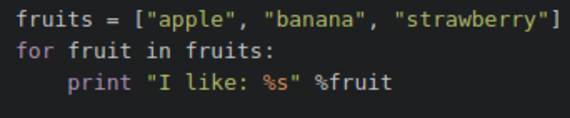
\includegraphics[height = 1.4cm]{forLoop.pdf} $\,$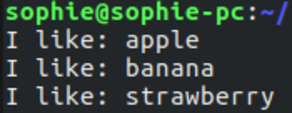
\includegraphics[height = 1.4cm]{forLoop_Output.pdf}\\
	while-loop: \\
		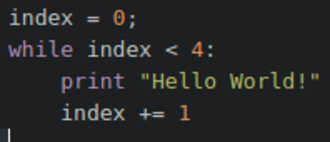
\includegraphics[height = 1.6cm]{whileLoop.pdf}$\,$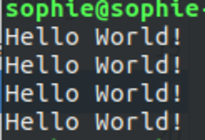
\includegraphics[height = 1.6cm]{whileLoop_Output.pdf}
	
\end{frame}
\begin{frame}
\frametitle{Examples}
	
	for-loop using \texttt{range()}:\\
		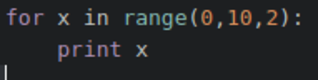
\includegraphics[height = 1.3cm]{forLoopRange.pdf} $\,$
		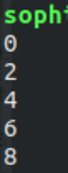
\includegraphics[height = 2cm]{forLoopRange_Output.pdf} \\
	The \texttt{range()} method creates a list with the parameters \texttt{(begin, end, step)}, where the end-value is not included! Default values are: \texttt{begin = 0} and \texttt{step = 1}, thus \texttt{range(4)} would create the list \texttt{[0,1,2,3]}.
		
	
\end{frame}


\begin{frame}
\frametitle{Exercises}
	\begin{itemize}
		\item Write the program \texttt{Faculty.py} that calculates the faculty of a certain number!
		\item Write the program \texttt{FibonacciSeries.py} that returns the Fibonacci Series! Use a list to store your result beginning with \texttt{Fibonacci = [0,1]}, the series should not exceed 10,000.
		\item Calculate the sum of all even numbers in your Fibonacci Series! You can reuse your code from exercise one.
	\end{itemize}
	There are many more mathematical problems or "number games" on \url {https://projecteuler.net/archives} you can solve with the few programming skills (but sometimes a lot of logical thinking) you have achieved here!
\end{frame}

\section{Functions}

\begin{frame}
\frametitle{Functions}
	You can organize code, that performs a single action with help of functions. This makes your code more readable and reusable. \\ You already saw a lot of "build-in" functions, like the \texttt{print} statement or the methods to manipulating lists, like \texttt{max()}. \\\ You can easily define your own functions using the \texttt{def} keyword:\\
		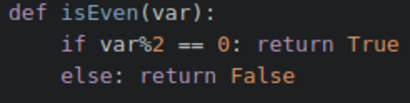
\includegraphics[height = 1.3cm]{isEvenFunc.pdf}\\
	And calling your function: \\
		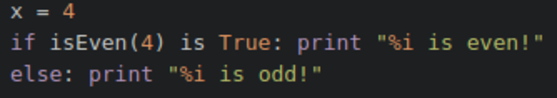
\includegraphics[height = 1.3cm]{FunctionUse.pdf}	 
\end{frame}


\begin{frame}
\frametitle{Exercises}
	\begin{itemize}
		\item Rewrite your \texttt{Faculty.py} program with a function \texttt{faculty(n)}!
		\item Write the function \texttt{faculty(n)} \textit{recursive}. This means that the function calls itself! Take care of defining an end condition (like \texttt{faculty(0)} returns 1) , otherwise you get stuck in an infinite loop! \\
		\begin{columns}[T]
		\begin{column}[T]{6cm}
			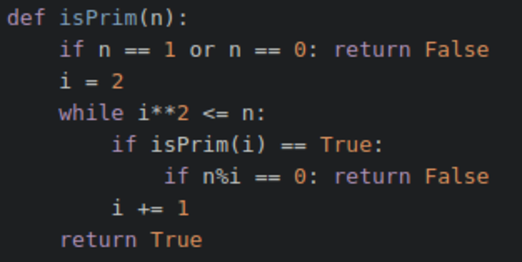
\includegraphics[width = 1\textwidth]{recursivePrim.pdf}
		\end{column}
		\begin{column}[T]{4cm}
			Example: \\
			Recursive function to calculate wether n is a prime number! 
		\end{column}
		\end{columns}
	\end{itemize}
\end{frame}

\section{Modules}

\begin{frame}
\frametitle{Modules}
	For the purpose of organize and reuse your code you can create \textit{Modules} which are basically files containing Python code like functions, variables or \textit{classes}. You can \textit{import} such modules (or single functions) using the \texttt{import} statement:
	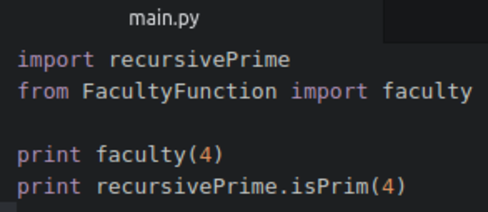
\includegraphics[width = 0.5\textwidth]{ImportStatements.pdf}
	\begin{alertblock}{Directory path}
		Your main method and modules must be in the same directory or you have to define a PYTHONPATH.
	\end{alertblock}
\end{frame}
	
	\subsection{Namespaces}
	
\begin{frame}
\frametitle{Namespaces}
	\begin{columns}[T]
		\begin{column}[T]{5.5cm}
			To avoid typing the module name before each function you imported with the \texttt{import} statement or to confuse different functions with similar names, you can use \textit{namespaces}. \\ Or you can import all items from one module into the current namespace using * (although this is not recommended and should be used  wisely)
		\end{column}
		\begin{column}[T]{5cm}
			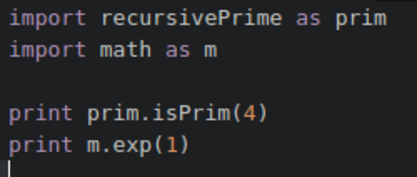
\includegraphics[width = 1\textwidth]{Namespaces.pdf} \\
			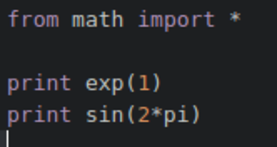
\includegraphics[width = 0.8\textwidth]{StarImport.pdf}
		\end{column}
		\end{columns}
\end{frame}

	\section{Command Line Arguments}

\begin{frame}
\frametitle{Command Line Arguments}
	For a convenient use of your programs you wouldn't want to open your python file, change the variables, save the file and then run it over the command line. Instead it would be better to run the code and define the variables over the command line: \\ $\,$ \\
	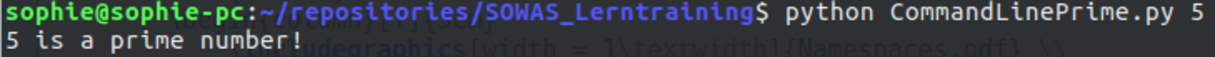
\includegraphics[width = 1\textwidth]{CommandLinePrime.pdf} \\
	This works with the \texttt{sys}-module, which you can easily import. This system module provides the list \texttt{sys.argv} which contains command line arguments as strings. \\ Another way is to read the keyboard input during runtime of your program using the \texttt{raw\_input} or \texttt{input} methods.
\end{frame}

\subsection{sys module}

\begin{frame}
\frametitle{sys-module example}
	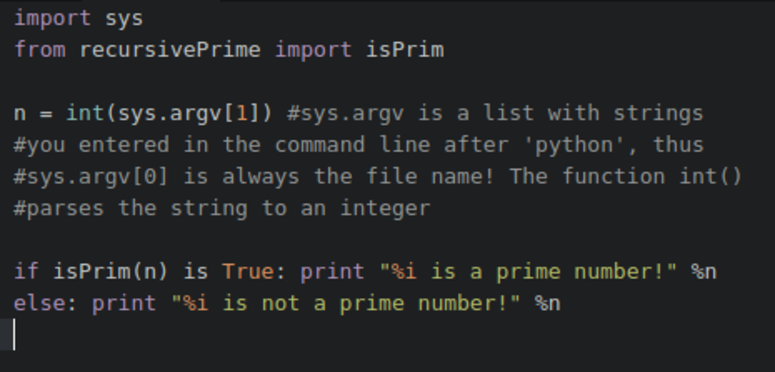
\includegraphics[width = 1\textwidth]{SysExample.pdf} 
\end{frame}


\begin{frame}
\frametitle{Exercises}
	\begin{itemize}
		\item Write a new command line based faculty program using the sys module! Import your old \texttt{faculty} function to calcuate it!
		\item Import the math module, and do some random calculation using its member functions. You can find them in the python documentary: \url{https://docs.python.org/2/library/math.html}
	\end{itemize}
\end{frame}

\section{Files}

\begin{frame}
\frametitle{Open files}
	Using the \texttt{open}-function to open files in read (r), write (w) or append (a) modus:
	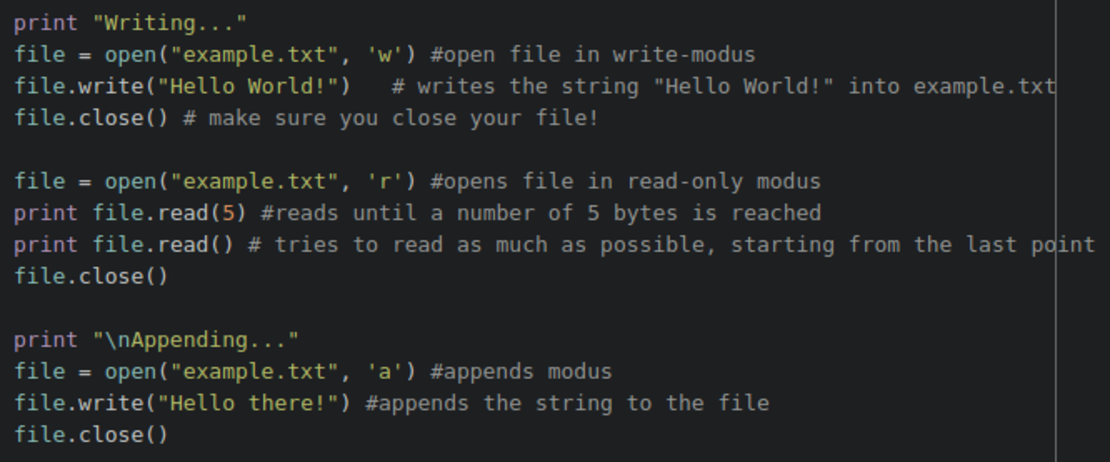
\includegraphics[width = 1\textwidth]{openFiles.pdf}
\end{frame}

\begin{frame}
\frametitle{Open files}
	\begin{alertblock}{Write-Modus}
	If you open your file in write modus it overwrites the file if it exists! Otherwise it creates a new one.
	\end{alertblock}
	\begin{itemize}
		\item You can use the modus \texttt{r+} or \texttt{w+} for reading AND writing
		\item You can set the position in your file using \texttt{file.tell()} which returns the position in your file, and \texttt{file.seek(offset, from)}. Where \texttt{offset} denotes the number of bytes, and \texttt{from} specifies from where the bytes are moved
		\item You can even delete files or make directories using the \texttt{os} module: \\ \url{https://www.tutorialspoint.com/python/python_files_io.htm}
	\end{itemize}
\end{frame}

\section{Matplotlib}
\begin{frame}
\frametitle{Matplotlib}
	\begin{itemize}
		\item Matplotlib is a plotting library. You can import it with the import statement! (Maybe you have to install it first)
		\item We are going to use the \texttt{pyplot} module which provides MATLAB-like interfaces and functions for simple plotting
		\item We also need the \texttt{NumPy} package in particular to get a real-valued \texttt{range} function, called \texttt{numpy.arange()}, but it's very useful for example for n-dimensional arrays, too!
	\end{itemize}
\end{frame}

\begin{frame}
\frametitle{Simple plot}
	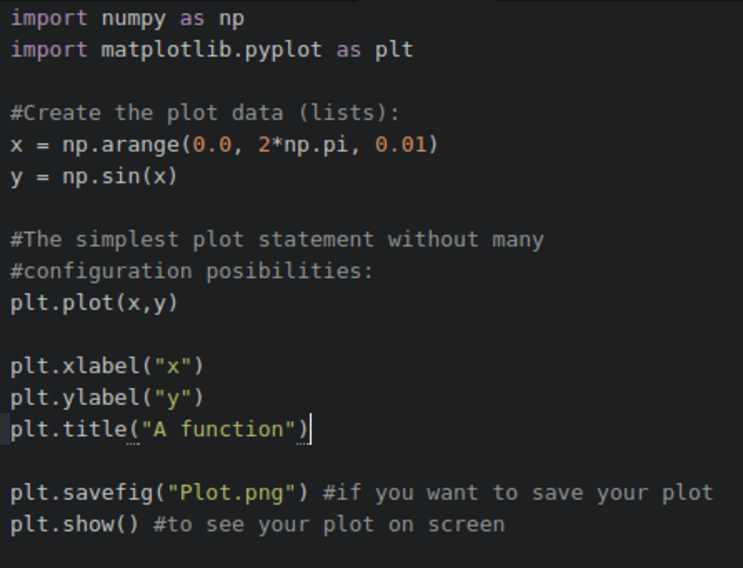
\includegraphics[width = 0.8\textwidth]{SimplePlot.pdf}
\end{frame}

\begin{frame}
\frametitle{Matplotlib}
	\begin{itemize}
		\item There are many more options you can set for your plots, like the range, colours or point-plots, a legend, some arrows and text boxes,...
	 	\item There are many other plots functions like: contour-plots, histograms, 3D-plots, polar plot, scatter plots,...
	 	\item You can use \texttt{TeX} statements in your plots using the \$-environment
	 	\item The best practice is to search for an example which is almost what you need and then to change it so that it fits for your purpose!
	 	\item If you want to plot your data with a ``lighter'' tool, you can use \texttt{gnuplot}! \url{http://www.gnuplot.info/}
	\end{itemize}
\end{frame}

\begin{frame}
\frametitle{Exercises}
	\begin{itemize}
		\item Implement an Euler integration for $\partial_t f(t) = f(t)$ with a step size of $\Delta t = 0.1$! Plot your numeric result as well as the analytic one using \texttt{np.exp()} in one plot to compare them! In this case, the Euler method is:
		\begin{align}
		f_{\mathrm{n+1}} = f_{n} + \Delta t \cdot f_{n}
		\end{align}
		Where $f_{\mathrm{n}}$ denotes the old solution state and $f_{\mathrm{n}+1}$ the new one, after one time step $\Delta t$. Thus, you can calculate $f_{1}$ using the initial values:
		\begin{align}
		f_{1} = f_{0} + \Delta t \cdot f_{0}
		\end{align}
		And $f_2$ can be calculated with $f_1$ and so on.
		
	\end{itemize}
\end{frame}


\begin{frame}
\frametitle{Exercises}
	\begin{itemize}
		\item Use $f(0) = f_0 = 1$ as initial condition and a final time of $T = 5.0$!
		\item Store your result of each time step in a list until a final time of $T= 5.0$ is reached. (Hint: use the \texttt{append()} method)
		\item Plot the analytic and numeric result after you reached the final time $T$ in your Euler calculation. You can plot two functions in one plot by simply using the plot statement \texttt{plt.plot()} twice.
		\item Store your results in a file (using a reasonable format) and save your plot! Use \textbackslash\texttt{n} and \textbackslash\texttt{t} to make a newline or a horizontal tab.
		
	\end{itemize}
\end{frame}

\section{Polyfit}
\begin{frame}
\frametitle{Polynomial fit with numpy}
	Numpy provides a function for polynomial curve fitting based on the minimalization of the squared errors between the polynomial and your points. \\If you store your points in a \texttt{numpy array} you could fit them as follows:
	%TODO Picture of curve fit!
\end{frame}


\section{Literature}
\begin{frame}
\frametitle{Some literature and useful websites}
	\begin{itemize}
		\item This tutorial and some advanced methods: \url{https://www.tutorialspoint.com/python/python_lists.htm}
		\item Book: \textit{A Primer on Scientific Programming with Python}, Hans Petter Langtangen, you can find it in our library, too!
		\item No matter what problem you have, someone had it before: \url{https://stackoverflow.com/}
		\item Python documentation: \url{https://www.python.org/} and matplotlib: \url{https://matplotlib.org/} use the examples and change them according to your wishes!
		\item If you love mathematical problems: \url{https://projecteuler.net/}
		\item My solutions to this exercises: \url{https://github.com/sophieaerdker/SOWAS_Lerntraining}
	\end{itemize}
\end{frame}


\end{document}